\documentclass{article}

\usepackage[utf8]{inputenc}
\usepackage[brazil]{babel}
\usepackage{amsmath}
\usepackage{amsfonts}
\usepackage[section]{placeins}
\usepackage{booktabs}
\usepackage{multirow}
\usepackage{listings}
\usepackage{booktabs}
\usepackage[title]{appendix}

\usepackage{caption}

\usepackage{hanging}
\usepackage{graphicx}

\usepackage{natbib}

% Commands --------------------------------------------------------------------

\newcommand\indep{\protect\mathpalette{\protect\independenT}{\perp}}
\def\independenT#1#2{\mathrel{\rlap{$#1#2$}\mkern2mu{#1#2}}}

\setlength{\parskip}{0.5em}

\def\arraystretch{1.5}

% Document basics -------------------------------------------------------------

\title{Métodos Numéricos - Lista 02}
\author{Samuel de S. Barbosa}
\date{Abril 2018}

\begin{document}

\maketitle

\section*{}

Nesta lista vamos solucionar o modelo de \textit{Real Business Cycles} (RBC) usando diferentes
técnicas de iteração da função valor.


\subsubsection*{Preferências}

$$ U(c) = \mathbb{E}_0 \sum_{t=0}^{\infty} \beta^t u(c_t) $$

$$ u(c_t) = \frac{c^{1-\mu}-1}{1-\mu}$$
$$\mu = 1/(1+r)$$

\subsubsection*{Tecnologia}

$$Y_t = z_t F(K_t, N_t) = z_t K_t^\alpha N_t^{1-\alpha}$$

$$ \log z_t = \rho \log z_{t-1} + \epsilon_t $$

$$ \varepsilon_t \sim N(0, \sigma^2) $$

\subsubsection*{Calibração}

$$\beta = 0.987, \,\,\,\,\, \mu=2, \,\,\,\,\,  \alpha=0.3, \,\,\,\,\,  \delta=0.012, \,\,\,\,\,  \rho=0.95, \,\,\,\,\, \sigma=0.007$$

\newpage


% ----------------------------------------------------------------------------------------------------------------------------------------
\subsubsection*{1. Escreva o problema do planejador na forma recursiva}

O problema do planejador consiste em maximizar $U(c)$ sujeito à restrição de
factibilidade $Y_t = C_t + S_t$ e à lei de movimento do capital 
$K_{t+1} = (1-\delta)K_t + S_t$.

Podemos escrever este problema na forma recursiva como

\begin{equation}
\begin{aligned}
 & V(k,z) = \max_{k^{\prime}, \, c} & & u(c) + \beta \mathbb{E} V(k^{\prime},z^{\prime}). \\
 & \text{s.a.} & & c = y - s \\
 &             & & k^{\prime} = (1-\delta) k + s
\end{aligned}
\end{equation}


Equivalentemente,

\begin{equation}
\begin{aligned}
 & V(k,z) = \max_{k^{\prime} \geq 0} & & u(zk^\alpha + (1-\delta)k - k^{\prime}) + \beta \mathbb{E} V(k^{\prime},z^{\prime})
\end{aligned}
\end{equation}


% ----------------------------------------------------------------------------------------------------------------------------------------
\subsubsection*{2. Assuma que não há incerteza, i.e., $\sigma = 0$. Derive a equação de Euler e encontre o capital de estado estacionário $k_{ss}$.}



Da condição de otimalidade e Teorema do Envelope obtemos a eq. de Euler:


\begin{equation}
\begin{aligned}
u^{\prime}(c) & = & & \beta  \mathbb{E} [ \frac{\partial}{\partial k^{\prime}} V(k^{\prime},z^{\prime})] \\
      & = & & \beta  \mathbb{E} [u^{\prime}(c^{\prime}) (\alpha z k^{\alpha-1} + 1 - \delta)].
\end{aligned}
\end{equation}


No estado estacionário, sem incerteza, temos $c^{\prime}=c=c_{ss}$ e $k^{\prime}=k=k_{ss}$. 

Além disso, 

\begin{equation}
\begin{aligned}
&  &\log(z_t)  = \rho \log(z_{t-1}) + \epsilon_t \\
&     \implies  & (1-\rho L) \log(z_t) = \epsilon_t = 0 \\
&     \implies  &  \log(z_t) =  0 \\
&     \implies &  z_t =  1. \\
\end{aligned}
\end{equation}

Logo

\begin{equation}
\begin{aligned}
1 & = & & \beta (\alpha k_{ss}^{\alpha-1} + 1 - \delta)  \iff \\
k_{ss}^{1-\alpha} & = & & \frac{1-\beta(1-\delta)}{\alpha \beta} \iff \\
k_{ss}            & = & & \left[ \frac{1-\beta(1-\delta)}{\alpha \beta} \right] ^ {\frac{1}{\alpha-1}}
\end{aligned}
\end{equation}

% ----------------------------------------------------------------------------------------------------------------------------------------
\subsubsection*{3. Resolva o problema utilizando método de iteração da função valor.}

Para a choque de TFP, vamos utilizar o método de Tauchen (1986) com
7 pontos. Para o grid de capital, usaremos 500 pontos linearmente espaçados
no intervalo $[0.75 k_{ss}, 1.25 k_{ss}]$.

Utilizando o método da força bruta como benchmark, obtemos a seguinte solução:

\begin{figure}[h!]
  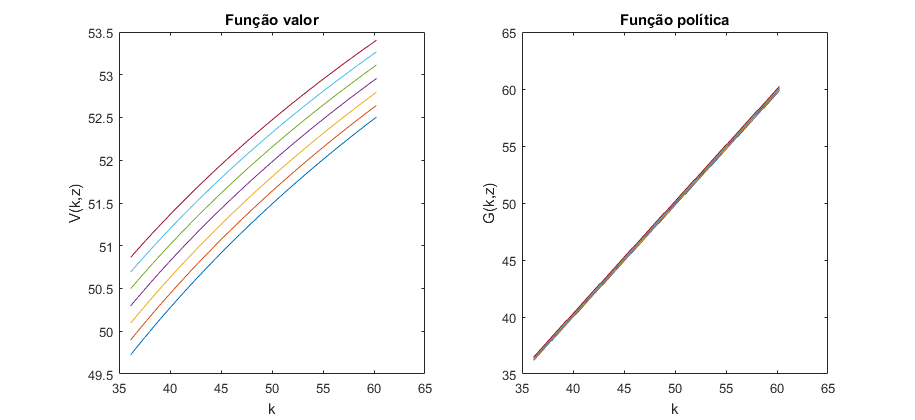
\includegraphics[width=\linewidth]{graf1.png}
\end{figure}

O tempo necessário para resolver o problema utilizando a força bruta (de forma vetorizada) foi de
14,73 segundos.

Como a função política é crescente no capital, podemos explorar essa
monotonicidade  para tentar obter uma solução mais rápida. Dada a primeira
iteração no método da força bruta, sabemos que a escolha ótima de capital
estará restrita ao intervalo $[k_1, k_{\max}]$. Ao restringir a maximização a
este intervalo, obtemos a solução em 21,79 segundos. Embora este método reduza
o tempo da solução não vetorizada, implementá-lo no algoritmo vetorizado
causou, de fato, uma perda de eficiência.

Em seguida, podemos explorar a concavidade da função valor. A concavidade nos
permite obter a solução somente observando a diferença da função valor
estimada entre pontos  consecutivos no grid. Utilizando esta técnica obtemos a
solução em 20,13 segundos, um tempo similar ao obtido explorando-se a
monotonicidade, porém não mais eficiente do que a força bruta vetorizada.

\subsubsection*{4. Refaça o item anterior usando o acelerador. Isto é, só
realize a maximização em algumas iterações (10\% delas, por exemplo). Compare
os resultados com o item anterior.}

Utilizando a técnica do acelerador (10\%) com o método da força bruta
vetorizada, obtemos a solução em 9,50 segundos, reduzindo o tempo em 35,5\%,
um ganho considerável.

\subsubsection*{5. Para este item, refaça o problema usando múltiplos grids
(multigrid). Primeiro, resolva o problema usando um grid de 100 pontos, depois
500 e, finalmente, 5000. Para cada grid posterior, utilize a solução anterior
como chute inicial (você precisará interpolar). Compare com os itens
anteriores.}

No primeiro passo (100 pontos), utilizando apenas força bruta vetorizada,
obtemos convergência da $V_1$ em 0,28 segundos. Em seguida, utilizando a
interpolação de $V_1$ em um grid de 500 pontos,  obtemos $V_2$ em 7,27
segundos.

No último passo, interpolamos $V_2$ em um grid de 5000 pontos. Neste passo,
obtemos convergência em 46,25 segundos.

No total, obtemos a função valor em um grid com 5000 pontos em aproximadamente
54 segundos.

\subsubsection*{6. Para este item, resolva o problema usando o método do grid endógeno
(endogenous grid method). Compare com os itens anteriores.}

O método do grid endógeno convergiu em um segundo. Para verificar os resultados
obtidos calculamos os \textit{Euler Errors} em cada estado. O gráfico a
seguir mostra os resultados obtidos:


\begin{figure}[h!]
  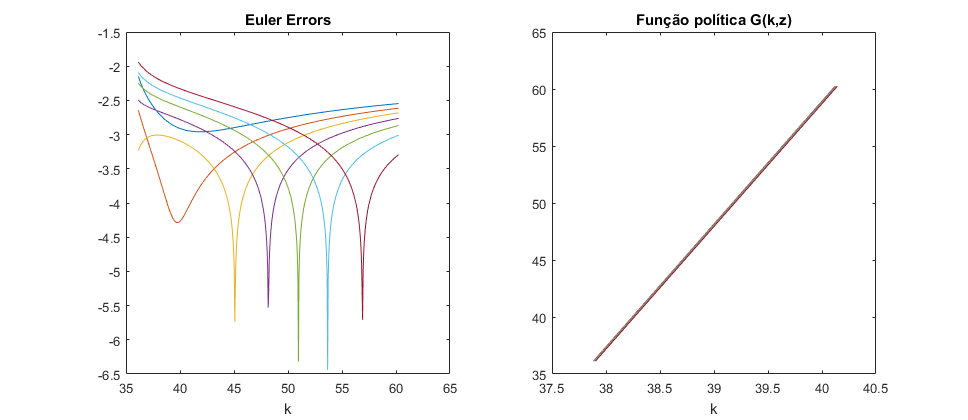
\includegraphics[width=\linewidth]{graf2.png}
\end{figure}


\end{document}